\newpage


\section{Istniejące metody partycjonowania grafów}
\label{sec:literature}

Rozbudowany podział metod został zaproponowany przez autorów artykułu - \cite{metis}
oraz \cite{1364754}
Zgodnie z ich analizą metody dzielimy na:
\begin{itemize}
    \item spektralne,
    \item rekursywne,
    \item geometryczne,
    \item wielopoziomowe.
\end{itemize}

\subsection{Metody spektralne}
Partycjonowanie spektralne daje dobre rezultaty i jest metodą w miarę często używaną
\cite{10.1137/0611030, 10.5555/147877.147902, improved_spectral}.
Podzbiór wierzchołków \(S \subset V\) grafu G nazywamy separatorem jeśli dwa wierzchołki w tym samym komponencie
grafu G są w dwóch różnych komponentach w grafie  \(G \setminus S\).

\begin{figure}[h]
    \centering
    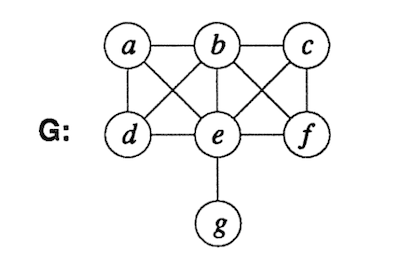
\includegraphics[width=0.3\linewidth]{images/separator}
    \caption{Separator wierzchołków d oraz c to \(\{b, e\}\).
    Źródło: \cite{MiTeThVa93}.}
    \label{im:separator}
\end{figure}

Metoda \cite{10.1137/0611030} będąca algorytmem spektralnym pokazuje algebraiczne podejście do obliczania
separatorów wierzchołków.
Artykuł \cite{10.5555/147877.147902} opisuje algorytm spectral nested dissection (SND).
Algorytmy te za pomocą znajomości spektralnych właściwości macierzy Laplaciana obliczają separatory wierzchołków w grafie,
które tworzą partycjonowanie grafu.
Artykuł \cite{improved_spectral} mówi o nowatorskim rozwinięciu metody spektralnej pod kątem umożliwienia podziału
obliczeń na cztery bądź osiem części na każdym etapie rekursywnej dekompozycji.
Są to jednak wszystko metody kosztowne z racji na
obliczanie wektorowa własnego odpowiadającego drugiej najmniejszej wartości własnej (Fielder wektor).
Istnieją udane próby ulepszenia czasu wykonania tych metod, które polegają na liczeniu Fielder wektora poprzez
algorytm wielopoziomowy - MSB \cite{fast_multilevel}. Jednak nawet te metody wciąż charakteryzują się wysoką złożonością.


\subsection{Metody rekursywne}

Są to metody często prostsze w implementacji, jednak nie sprawdzają się tak dobrze w kontekście bardziej
skomplikowanych problemów głównie ze względu na to, że mają zachłanną naturę.
Metoda \cite{recursive} zakłada, że dzielimy siatkę na liczbę obszarów,
która jest równa potędze liczby dwa. Ta metoda potrafi także dzielić siatkę wedle możliwości obliczeniowych
poszczególnych rdzeni procesora. Czasami metody rekursywne są implementowane jako faza metod
bisekcji spektralnej \cite{10.1137/0611030}. Przykłady działania partycjonowania rekursywnego przedstawione są na rysunkach
\ref{im:recursive_partitioning} oraz \ref{im:rec_partitioning}.

Specyfika tych metod polegająca na dzieleniu grafu na coraz mniejsze
części sprawia, że nie jesteśmy w stanie uwzględniać części niepodzielnych, lub rozwiązanie tego problemu byłoby skomplikowane.


\begin{figure}[h]
    \centering
    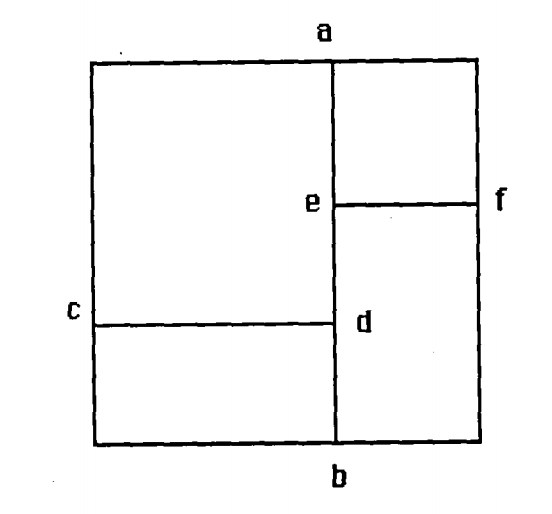
\includegraphics[width=0.3\linewidth]{images/recursive}
    \caption{Przedstawia partycjonowanie rekursywne na głębokości wynoszącej 2. Linia partycjonowania a-b, która została stworzona
    przez partycjonowanie poziomu 1 jest podzielona na 3 segmenty przez dwie linie partycjonowania poziomu drugiego:
    c-d, e-f. Źródło: \cite{recursive}}
    \label{im:recursive_partitioning}

    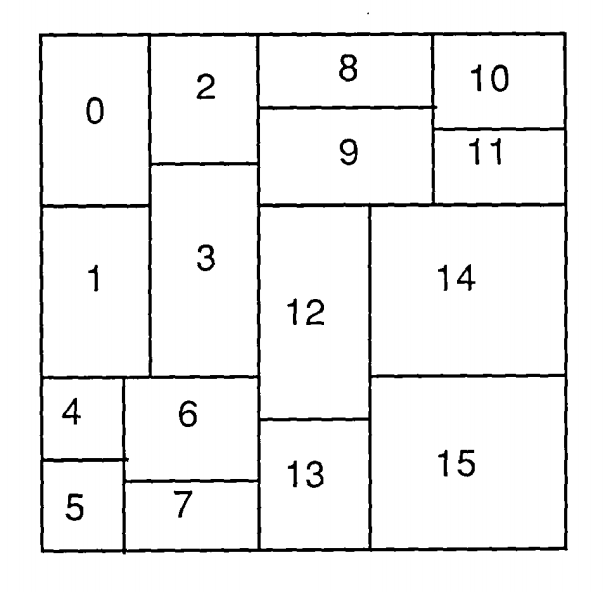
\includegraphics[width=0.3\linewidth]{images/recursive-part}
    \caption{Metoda rekursywna - binarna dekompozycja dla 16 procesorów. Najpierw tworzone jest wertykalne cięcie,
        które gwarantuje, że prawy i lewy obszar
        zawiera połowę pracy do wykonania (lub takie, które jest jak najbliżej takiego podziału). Jeśli dostępne
        są 4 procesory to każdy z dwóch segmentów partycjonowany jest horyzontalną linią, która spełnia te same założenia
        jak ta dla pierwszego wertykalnego cięcia. Procedura jest kontynuowana na zmianę wykorzystując wertykalne i
        horyzontalne cięcie aż do otrzymania podziału na oczekiwaną liczbę obszarów. Źródło: \cite{recursive}}
    \label{im:rec_partitioning}
\end{figure}

\newpage
\subsection{Metody geometryczne}

\begin{wrapfigure}{r}{0.41\textwidth}
    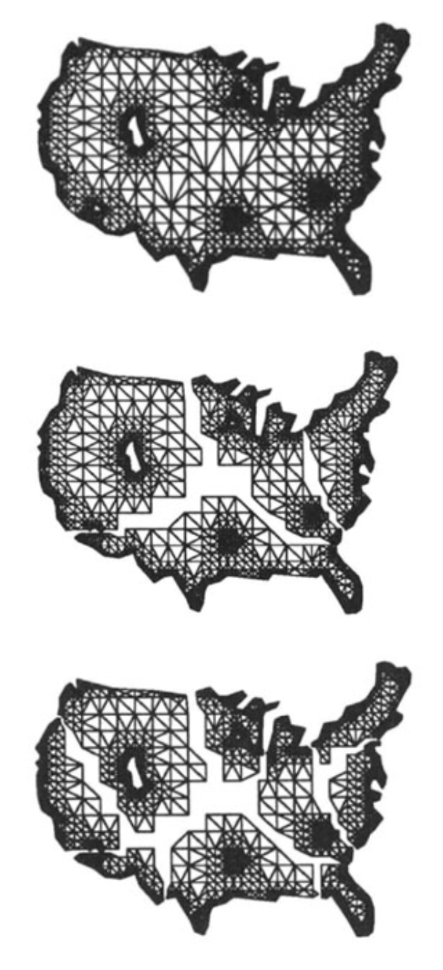
\includegraphics[width=\linewidth]{images/recursive-partitioning}
    \caption{Rekursywne partycjonowanie mapy USA - pierwszy obrazek od góry - za pomocą algorytmu z artykułu \cite{MiTeThVa93}.
    Dwa następne obrazki prezentują rezultat. Dane geometryczne używane są do obliczenia separatorów.}
\end{wrapfigure}


Inną klasą metod są metody geometryczne
\cite{Miller1994ACP, Raghavan93lineand, 185417, MiTeThVa93, NourOmid1987SolvingFE}.
Używają danych geometrycznych o grafie w celu znalezienia dobrego partycjonowania.
Ich cechą charakterystyczną jest relatywnie krótki czas wykonania, natomiast gorsze rezultaty podziału niż metody spektralne.
Najlepsze wyniki spośród wyżej wymienionych metod prezentują \cite{185417, MiTeThVa93}.
W artykule \cite{185417} zaproponowane klasę grafów zwaną k-overlap graphs. Dla grafów k-overlap osadzonych w d wymiarach
 \cite{wiki:Graph_embedding} udowadniają istnieje separatora wielkości \(O(k^{1/d}D^{{d-1}/d})\).
Oznacza to, że dla grafu o N wierzchołkach istnieje podzbiór
wierzchołków o wcześniej wymienionej wielkości, który po usunięciu rozłącza graf na dwie podobnej wielkości części.
Wyniki w tym artykule unifikują kilka wcześniejszych wyników dla obliczania separatorów.
Ponadto autorzy proponują rozwiązanie, które oblicza separatory w czasie liniowym.
W artykule \cite{MiTeThVa93} opisano efektywną metodę partycjonowania siatek niestrukturalnych, która występują w metodach
elementów skończonych i różnic skończonych. Podejście to wykorzystuje strukturę geometryczną danej siatki i znajduje
dobre partycjonowanie w czasie \(O(n)\). Można je aplikować do siatek w dwóch i trzech wymiarach. Ma zastosowanie
w wydajnych algorytmach sekwencyjnych i równoległych do rozwiązywania rozbudowanych problemów w obliczeniach naukowych.
Charakterystyką metod geometrycznych jest to, że z powodu losowej natury wymagane jest wielokrotne użycie algorytmu
(od 5 do 50 razy) aby uzyskać wynik porównywalny z metodami spektralnymi.
Wielokrotnie wywołanie zwiększa czas otrzymywania rezultatu, natomiast jest
on wciąż niższy od metod spektralnych. Metody geometryczne są aplikowalne tylko w przypadku kiedy dostępne
są współrzędne wszystkich wierzchołków w grafie. Dla wielu dziedzin problemów (programowanie liniowe, VLSI),
nie otrzymujemy współrzędnych wraz z grafem. Istnieją algorytmy, które są w stanie obliczyć współrzędne dla
wierzchołków grafu \cite{Chan95geometricspectral} wykorzystując metody spektralne ale są bardzo kosztowne i dominują czas potrzebny
na samo partycjonowanie grafu.
Implementacje tego typu metod nie znalazły się wśród algorytmów state-of-the-art dla problemu partycjonowania grafów,
więc nie były brane pod uwagę w kontekście niniejszej pracy.

\newpage

\subsection{Metody wielopoziomowe}

Istnieje wiele implementacji metod wielopoziomowych: \cite{metis, jostle, Bui1993AHF, 103500, 185177, 279334, inproceedings, 129970, 10.1145/165939.165942}.
Cechą charakterystyczną tego podejścia jest redukcja
wielkości grafu poprzez łączenie wierzchołków i krawędzi, następnie dzielenie zmniejszonego grafu na partycje, ostatnią fazą
jest przywrócenie początkowego grafu zachowując podział.
Często graf zmniejszany jest aż liczba wierzchołków nie osiągnie
liczby partycji, którą chcemy otrzymać \cite{1364754}, a fazie przywracania grafu do początkowej wielkości towarzyszy
algorytm, którego celem jest ulepszanie podziału \cite{article, 10.5555/800263.809204}.
Algorytm ten, bazując na zmniejszonym
grafie, niesie za sobą niższy koszt obliczeniowy.
Jego działanie polega na zmniejszaniu długości granic pomiędzy partycjami z jednoczesnym zachowaniem ich wielkości.
Na tym etapie może także zostać dodana faza balansowania, która stopniowo zmniejsza różnice w wielkości pól pomiędzy
obszarami.
Metody te zostały stworzone z myślą o zmniejszeniu czasu patrycjonowania kosztem jego jakości.
Obecnie dają jednak bardzo dobre rezultaty również w kwestii jakości podziału.
Późniejsze prace w dziedzinie tych algorytmów pokazały, że dają one lepsze rezultaty niż metody spektralne \cite{metis}.
Biblioteki jak Party \cite{1364754}, Metis \cite{metis}, Jostle \cite{jostle}, Chaco \cite{inproceedings},
dające state-of-the-art wyniki w kwestii jakości partycjonowania najczęściej bazują na schemacie wielopoziomowym
\cite{inproceedings}.

\begin{figure}[h]
    \centering
    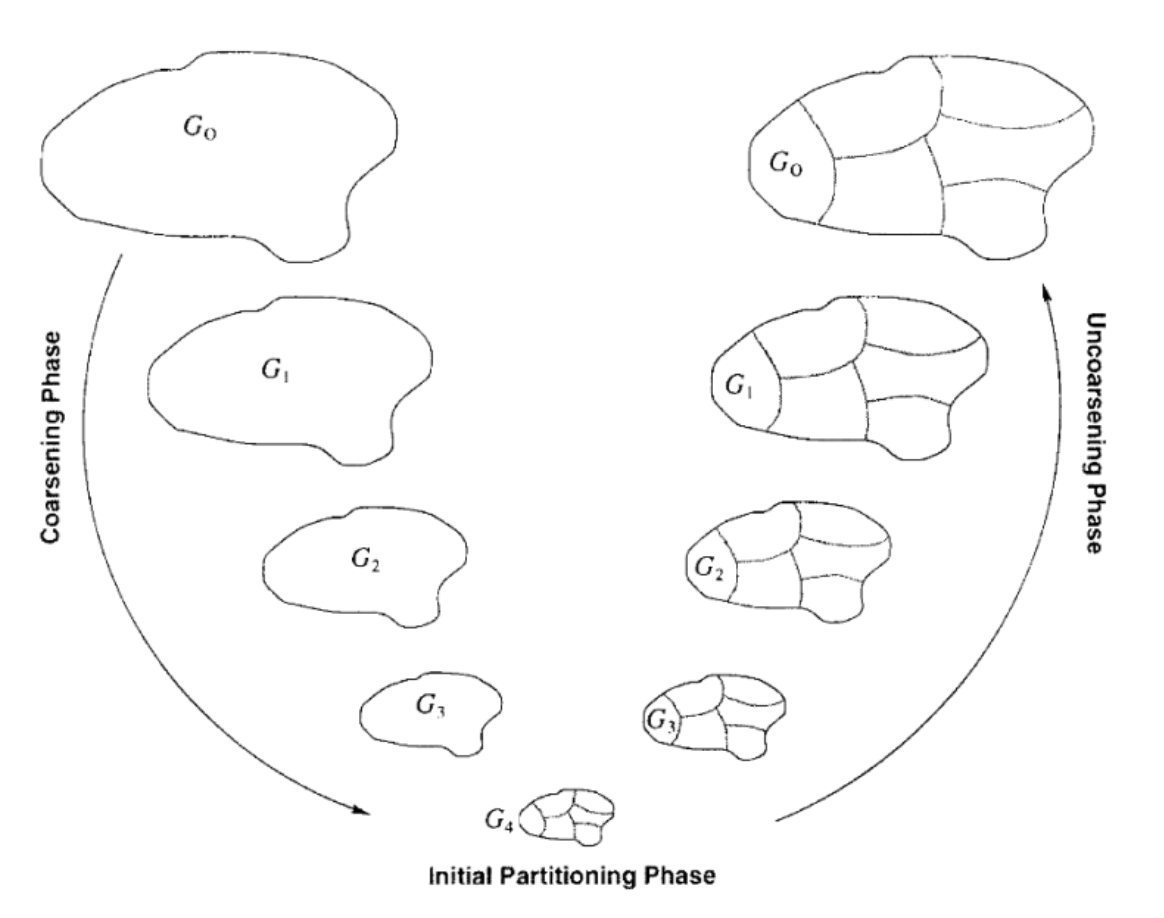
\includegraphics[width=0.9\linewidth]{images/coarsening}
    \caption{Wielopoziomowe partycjonowanie grafu przedstawiające fazę zmniejszania grafu, następnie przypisanie
    partycji na zmniejszonym grafie, na końcu przywrócenie grafu do początkowej wielkości.
    Źródło: \cite{KARYPIS199896}.}
    \label{im:multilevel_partitioning}
\end{figure}


\subsection{Porównanie istniejących metod wielopoziomowych}

Wszystkie wyżej wymienione metody nie biorą pod uwagę problemu obszarów niepodzielnych oraz obszarów wyłączonych z obliczeń.
W związku z tym celem niniejszej pracy stało się znalezienie metody dającej możliwie najlepsze rezultaty w zakresie partycjonowania grafów oraz
dostosowanie jej do wyżej wymienionych rozszerzeń problemu partycjonowania.

Metody wielopoziomowe są najlepszym wyborem, z racji na to, że gwarantowały najlepsze wyniki partycjonowania.
Przykładów metod wielopoziomowych jest bardzo dużo \cite{metis, jostle, Bui1993AHF, 103500, 185177, 279334, inproceedings, 129970, 10.1145/165939.165942},
jednak skupiłem się głównie na tych, które dawały wyniki state-of-the-art. Były to biblioteki:
Party \cite{1364754}, Metis \cite{metis}, Jostle \cite{jostle}, Chaco \cite{inproceedings}.

\begin{figure}[h]
    \centering
    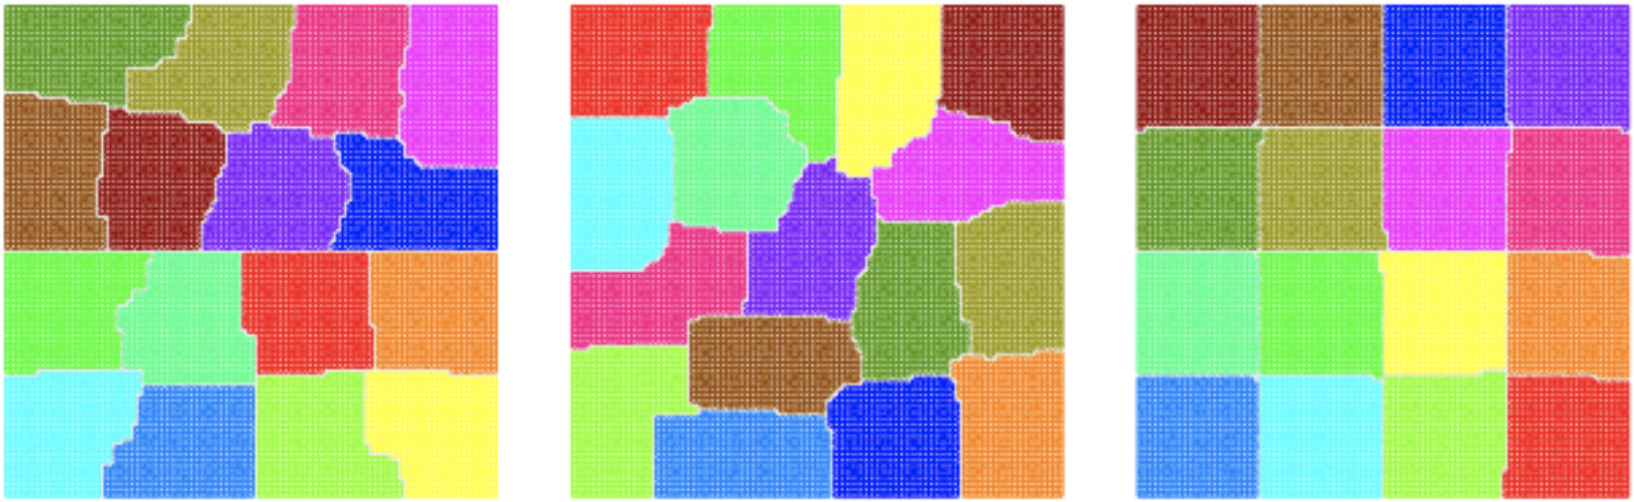
\includegraphics[width=0.7\linewidth]{images/libraries-comparision}
    \caption{Partycjonowanie siatki 100x100 na 16 obszarów. Od lewej - pmetis \cite{metis} uzyskuje edge-cut wynoszący
    688, następnie Jostle \cite{jostle} z wynikiem 695 oraz Party \cite{1364754} z wynikiem 615. Źródło: \cite{1364754}.}
    \label{im:partitioning_results}
\end{figure}

Do zmniejszenia grafu stosowane są różne warianty matching algorithm (algorytm do budowania skojarzeń w grafie).
Porównanie większości z nich można znaleźć w \cite{Analysis}.
Przykładowo biblioteka Jones oraz Bui \cite{Bui1993AHF} używam random weighted matching, natomiast Party \cite{1364754}
stosuje LAM matching \cite{weighted_maching}.
Ze względu na wymagania co do złożoności obliczeniowej wszystkie metody używają heurystyk.
Wszystkie z tych metod zmniejszają graf, jednak tylko Jostle i Party zmniejsza graf
aż do otrzymania liczby wierzchołków równej liczbie partycji, na które chcemy podzielić wejściowy graf.
Dzięki temu metoda partycjonowania, działająca na najmniejszym możliwym grafie, jest dużo prostsza niż w pozostałych metodach.
Kiedy graf jest zmniejszony, wierzchołki są przyporządkowywane do partycji a informacja na temat partycji jest propagowana
do wierzchołków na wyższych poziomach zgodnie z partycją ich reprezentantów na najniższym poziomie.
Ten proces prowadzi do partycjonowania początkowego grafu.
Faza zmniejszania grafu jest ponadto stosunkowo łatwa do zrównoleglenia \cite{KARYPIS199871}.
Fazą, która nie podlega zrównolegleniu jest faza ulepszania istniejącego podziału.
Najczęściej bazuje ona na metodzie Fiduccia-Mattheysesa \cite{10.5555/800263.809204},
która jest zoptymalizowaną pod kątem czasu działania heurystyką Kerninghan-Lin (KL) \cite{6771089}.
Artykuł \cite{6771089} podejmuje problem partycjonowania wierzchołków grafu, którego krawędzie mają
przyporządkowane wagi - koszt.
Jego celem jest ustanowienie podziału na obszary o wybranej wielkości wraz
ze zminimalizowaniem sumy kosztów na wszystkich granicach.
Artykuł \cite{10.5555/800263.809204} przedstawia heurystykę do poprawiania partycjonowania sieci.
Algorytm ten przesuwa pojedyncze komórki pomiędzy blokami wraz z utrzymaniem oczekiwanego rozmiaru bloków.
W przeciwieństwie do Metis i Jostle, faza ulepszenia partycjonowania używana przez bibliotekę Party bazuje na metodzie
Helpful-Sets (HS).
Heurystyka Helpful-Set wywodzi się z obserwacji teoretycznych wykorzystywanych do znajdowania górnych
granic szerokości bisekcji grafów regularnych \cite{10.1007/3-540-54345-7_64, MONIEN2006475}.
Szerokość bisekcji to minimalna liczba krawędzi, która musi zostać usunięta w celu podzielenia grafu na
dwie równej wielkości części, lub różniące się wielkością o maksymalnie jeden wierzchołek.
Party otrzymuje bardzo dobre wyniki stosując tę metodę \cite{10.1007/3-540-44842-X_6}, często uzyskując mniejszą długość
granic pomiędzy obszarami niż Metis czy Jostle, jednocześnie jest tylko trochę bardziej kosztowna obliczeniowo.
Heurystyka Helpful-Sets jest metodą bazującą na wyszukiwaniu lokalnym.
Zaczynając od początkowej bisekcji \(\pi\) dąży
do zminimalizowania długości granicy za pomocą lokalnie wprowadzanych zmian.
Najważniejsza różnica względem metody KL polega na tym że KL przemieszcza tylko pojedyncze wierzchołki,
natomiast HS zbiory wierzchołków.
Zarówno Party, Metis, jak i Jostle pozwalają na małe nierówności w kwestii wielkości obszarów co przekłada się na
mniejsze długości granic,
szczególnie na głębszych poziomach, kiedy przemieszczane są wierzchołki o dużych wagach - ciężko wtedy o otrzymanie
idealnie równych obszarów.

Biblioteka Party \cite{1364754} okazała się dawać najlepsze rezultaty w porównaniu do innych bibliotek dających wyniki
state-of-the-art.
Szczególną własnością Party była znacznie niższa długość granic w porównaniu do pozostałych bibliotek
(Rysunek \ref{im:partitioning_results}), co było bardzo ważne dla mojej pracy.
Dlatego to właśnie metodę z biblioteki
Party zdecydowałem się wybrać jako podstawę rozwiązania prezentowanego w niniejszej pracy.